\section{Desplazador de barril \label{sec:s1}}

\begin{center}
	\begin{minipage}{12cm}
		\begin{tcolorbox}[title=Actividad 1]
			Un desplazador de barril (“\textit{barrel shifter}”) es un circuito combinatorio que permite desplazar un dato de entrada tantas posiciones como se indique en su control. Investigar su funcionamiento y describir un desplazador de barril de 4 bits. Simular el circuito.
		\end{tcolorbox}	
	\end{minipage}
\end{center}

Un desplazador de barril (o \textit{barrel shifter}, en ingles) es un circuito digital que desplaza (o rota) los bits de una palabra de entrada un cierto número de posiciones especificado mediante un valor binario en unas lineas de selección. El desplazamiento se puede hacer en un sentido o en ambos por medio de otra variable de control. La forma más sencilla de lograr esto es mediante el uso de una serie de multiplexores donde una salida está conectada a la entrada del siguiente multiplexor en la cadena, de una manera específica que depende de la cantidad de desplazamiento especificado. \cite{Rouse_2017}

Un desplazador de barril consta de una serie de multiplexores. Cada multiplexor selecciona uno de los bits de entrada basándose en una señal de control del registro de cantidad de desplazamiento. Luego, la salida de cada multiplexor se conecta a la entrada del siguiente multiplexor de la cadena, formando un bucle. La salida del último multiplexor de la cadena es el valor desplazado.\cite{Mathur_2023} Por ejemplo, un \textit{barrel shifter} de 4 bits y con entradas A, B, C y D, puede ciclar el orden de los bits ABCD como DABC, CDAB o BCDA, en donde ningún bit se pierde. Esto muestra que se pueden cambiar todas las salidas hasta 3 posiciones a la derecha. \cite{Limones_2015}

Hay dos tipos de desplazadores de barril: el aritmético y el lógico.

\begin{itemize}
	\item \textbf{Desplazador aritmético}: Se utiliza para desplazar números binarios con o sin signo. Está diseñado para preservar el bit de signo del número al cambiar. Si el número que se está desplazando es un número con signo, el desplazador aritmético desplazará el bit de signo junto con los demás bits.
	\item \textbf{Desplazador lógico}: Se usa para desplazar sólo números binarios sin signo. No conserva el bit de signo del número al realizar el cambio.
\end{itemize}

Algunas aplicaciones del desplazador de barril son:

\begin{itemize}
	\item \textbf{Procesamiento de señales digitales}: Se utilizan para realizar operaciones rápidas de multiplicación y división. Por ejemplo, en una implementación de filtro FIR, se puede usar un desplazador de barril para cambiar los coeficientes del filtro según el orden del filtro.
	\item \textbf{Criptografía}: Se emplean para realizar operaciones bit a bit, como cifrado y descifrado. Por ejemplo, se puede utilizar un desplazador de barril para realizar un cambio circular en un valor binario para mejorar la seguridad del algoritmo de cifrado.
	\item \textbf{Arquitecturas de microprocesadores}: Se usan para cambiar el contenido de los registros, lo que permite una manipulación eficiente de los datos. Por ejemplo, en la arquitectura ARM, el desplazador de barril se utiliza para realizar operaciones de cambio y rotación en el contenido de los registros. \cite{Mathur_2023}
\end{itemize}

La visualización RTL del desplazador de barril en Verilog se muestra en la \autoref{fig:barrel_shifter_rtl}. Como se observa, la implementación se realiza utilizando solamente instancias de multiplexores, cuatro de ellos para el desplazamiento según la selección y uno extra para el sentido del desplazamiento. Las simulaciones se visualizan en la \autoref{fig:barrel_shifter_wave}, en donde se muestra que el dispositivo funciona de manera correcta, cargando un valor y rotándolo tanto a la izquierda como a la derecha.

En los Anexos se localiza la descripción del desplazador de barril. Al tratarse de un circuito combinatorio, la lista sensible tiene de argumento a todas las señales de entrada. Ahora bien, utilizando una estructura \textit{case}, se evalúo la cantidad de desplazamientos que se debía hacer y con el operador \textit{?} se seleccionó el sentido.

\begin{figure}[ht]
	\centering
	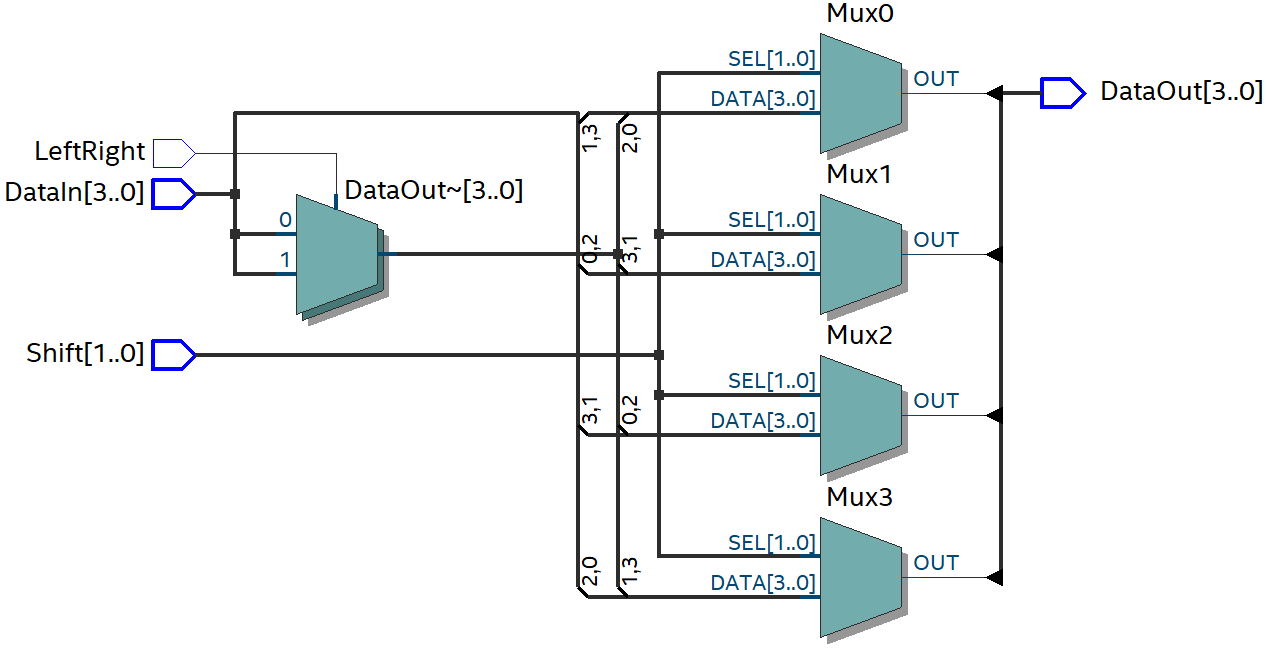
\includegraphics[scale=0.5]{Barrel_Shifter_RTL.png}
	\caption{Diagrama RTL del desplazador de barril de 4 bits. \label{fig:barrel_shifter_rtl}}
\end{figure}

\begin{figure}[ht]
	\centering
	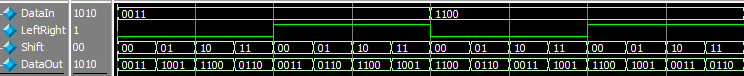
\includegraphics[scale=0.85]{Barrel_Shifter_Wave.png}
	\caption{Simulación del desplazador de barril de 4 bits con el visor de formas de onda de ModelSim. \label{fig:barrel_shifter_wave}}
\end{figure}